\begin{frame}{Par\'ametro U de Hubbard}
    Los orbitales \textbf{d} fuertemente correlacionados requieren una correcci\'on de la energ\'ia.
    \[
    E^{LDA+U} [\rho (r)]= E^{LDA} [\rho (r)] + 
    E^{Hubbard}[n_{mm^{\prime}}^{I\sigma}] - E^{dc}[n^{I\sigma}]
    \]
    Donde:
    
    \begin{itemize}
        \item $E^{LDA} [\rho (r)]$ funcional de la energ\'ia en LDA.
        \item $E^{Hubbard}[n_{mm^{\prime}}^{I\sigma}]$ correlaci\'on de los estados ocupados de los orbitales.
        \item $E^{dc}[n^{I\sigma}]$ energ\'ia de correlaci\'on, para evitar el doble conteo.
    \end{itemize}
\[
E^{LDA+U} [\rho (r)]= E^{LDA} [\rho (r)] + \sum _{I} \left[ \frac{U}{2} \sum 
_{m,\sigma \neq m^{\prime},\sigma ^{\prime}} n_{m}^{I\sigma} 
n_{m^{\prime}}^{I\sigma ^{\prime}} - \frac{U}{2} n^{I}(n^{I}-1) \right]
\]
\end{frame}

\begin{frame}
    {\bf C\'alculo de U: semi-emp\'irico}
    Se prueban varios valores de {\bf U} buscando que los resultados coincidan con datos experimentales.
    \begin{figure}[H]
        \centering
        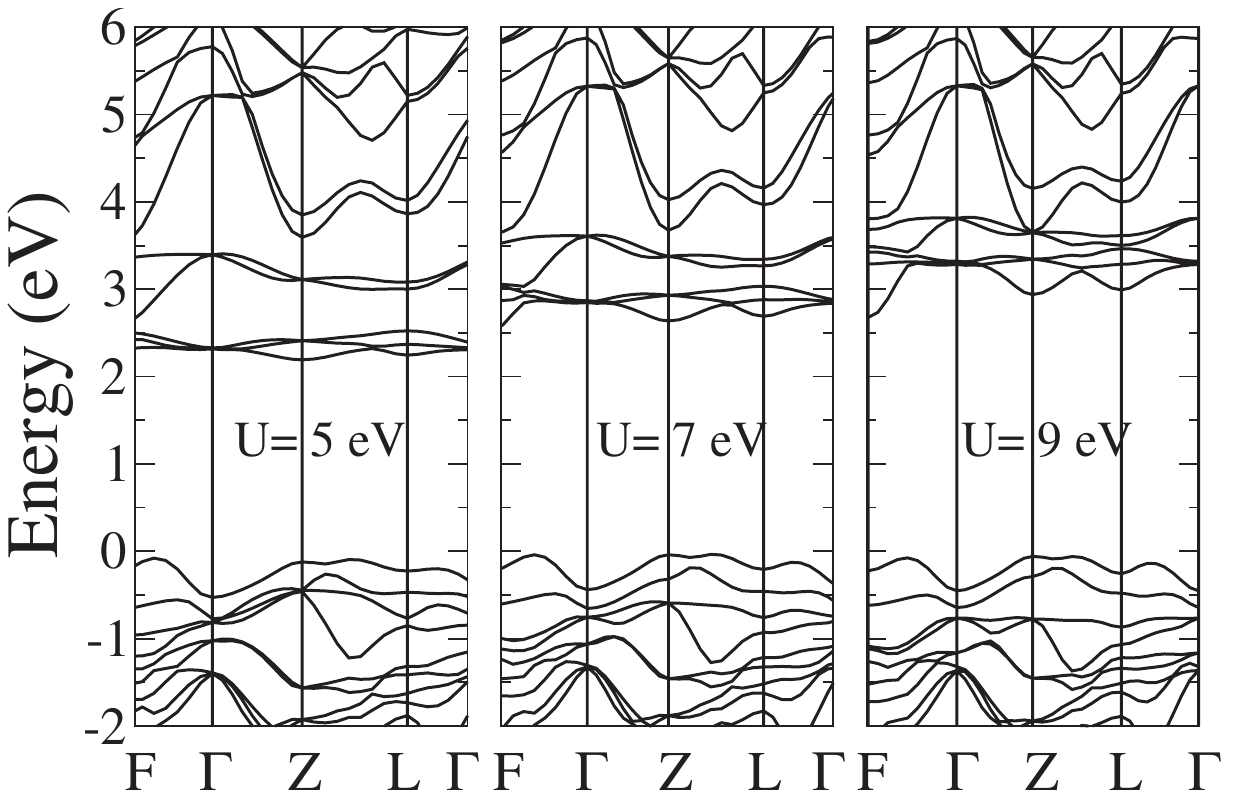
\includegraphics[width=0.6\textwidth]{contenido/teoria/img_teoria/hubbars.png}
        \caption{Estructura de bandas con diferentes valores de U. Sheng Ju et al. J. Chem. Phys. 130, 214708 (2009)}
    \end{figure}
\end{frame}

\begin{frame}
    {\bf C\'alculo de U: respuesta lineal}
    \begin{columns}[t]
        \column{0.5\textwidth}
        Se aplica una perturbaci\'on $\alpha$ en la energ\'ia de los estados {\bf d}.
        \[ U = \chi _{0}^{-1} - \chi ^{-1} \]
        donde: \[ \chi  = \frac{d n}{d \alpha } \]
        $\alpha$ es peque\~no y en un intervalo alrededor de cero.

        {\scriptsize Cococcioni and Gironcoli (2005)}        \column{0.5\textwidth}
        Procedimiento en Quantum ESPRESSO:
        \begin{itemize}
            \item C\'alculo scf sin perturbaci\'on.
            \item C\'alculo scf con cada valor de $\alpha$.
        \end{itemize}
    \begin{figure}[H]
        \centering
        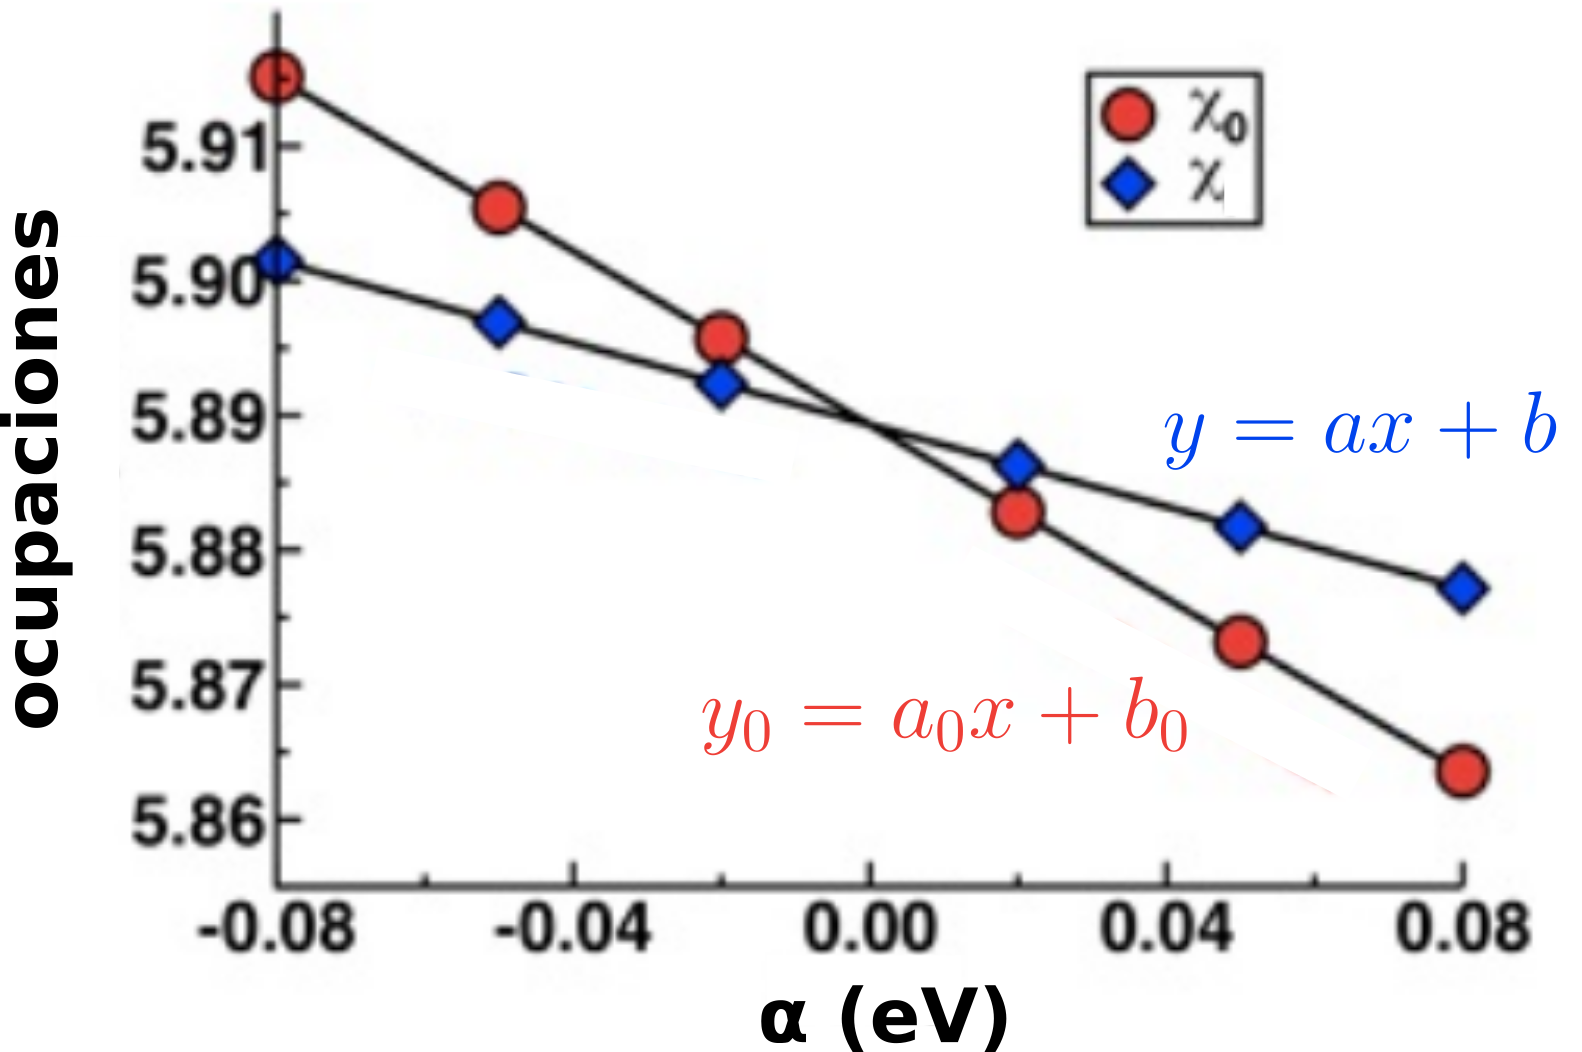
\includegraphics[width=1.0\textwidth]{contenido/teoria/img_teoria/RespuestaLineal.png}
    \end{figure}
\[ U = \chi _{0}^{-1} - \chi ^{-1} = 1/a_{0} - 1/a  \]
    \end{columns}
\end{frame}